\newpage
\section{Teilversuch 5: Quantitative Registrierung der Entladekurve eines Kondensators}
	Aus dem Handbuch des Oszilloskop\footnote{\url{cdn.rohde-schwarz.com/hameg-archive/HM1507-3_deutsch.pdf}} gibt es zwei verscheidene Quelle von Unsicherheiten:
	\begin{enumerate}
		\item Ablenkkoeffizienten (vertikal und horizontal) 
		\item Speicherauflösung
	\end{enumerate}
	Wir gehen davon aus, dass das Ablesen mittels des Cursors intern im Oszilloskop erfolgt. Somit spielt die Tolerenz bei den Ablenkkoeffizienten keine Rolle in den Daten. Folglich ist die Hauptunsicherheit die Speicherauflösung.

	Diesbezüglich ist die Speicherauflösung:
	\begin{center}
		\begin{tabular}{lrrr}
			\toprule
			& Auflösung & Einst. & $\Delta$ Wert	\\
			\textit{Einheit} & Punkte/Teilung & \_ / Teilung &  \\
			\midrule
			Vertikal & $25$ & \SI{1}{\volt} & $\pm \SI{0.02}{\volt}$ \\
			Horizontal & $200$ & \SI{200}{\milli\second} & $\pm \SI{1}{\milli\second}$ \\
			\bottomrule
		\end{tabular}
	\end{center}
	Da aber bei dem Ablesen von der Zeit nach $\SI{1}{\second}$ nur die erste Nachkommastelle gezeigt wurde, ist die Unsicherheit nach $\SI{1}{\second}$ viel größer und beträgt $\SI{0.05}{\second} = \SI{50}{\milli\second}$. 

	Somit haben wir als Messdaten:
	\begin{equation*}
		\begin{tabu}{l *{13}{r}}
			\toprule 
			t/\si{\milli\second} & 0 & 93 & 163 & 280 & 441 & 500 & 600 & 700 & 800 & 900 & 1000 & 1100 & 1200 \\
			\Delta t/\si{\milli\second} & 1 & 1 & 1 & 1 & 1 & 1 & 1 & 1 & 1 & 1 & 50 & 50 & 50  \\
			\midrule
			U_C/\si{\volt} & 3,93 & 3,29 & 2,93 & 2,33 & 1,73 & 1,57 & 1,29 & 1,09 & 0,88 & 0,720 & 0,60 & 0,520 & 0,440 \\
			\bottomrule
		\end{tabu}
	\end{equation*}
	mit $\Delta U = \SI{0.02}{\volt}$.

	Aus der Anleitung gilt:
	\begin{align}
		U_C &= U_0 \exp\left(-\frac{t}{RC}\right) && \Leftrightarrow && \ln U_C = \left(-\frac{1}{RC}\right)t + \ln U_0
	\end{align}
	Es ist aber wegen des Triggers so, dass der Kondesator bei $t = 0$ schon etwas entlädt hat, somit ergibt sich die modifizierte Gleichung:
	\begin{equation}
	  	\ln U_C = \left(-\frac{1}{RC}\right)t + \left(\ln U_0 -\frac{t_0}{RC}\right) \label{eqn:tv5eqn}
	\end{equation}
	Der entsprechende Fehler von $\ln U_C$ ist dann laut AMW:
	\begin{equation}
		\Delta (\ln U_C) = \frac{\Delta U_C}{U_C}
	\end{equation}
	$\ln (U_C/\si{\volt})$ wurde dann gegen die Zeit im \gnuplot{} geplottet und eine Kurveanpassung zur $$\ln (U_C/\si{\volt}) = mt + c$$ durchgeführt. 

	Im \gnuplot{} sind die Messpunkten für $t$ ins \si{\second} umgewandelt, sodass die Größeordunung der beiden Achse ähnlich sind. Diese Vorgehensweise hilft bei der Kurveanpassung. Die entsprechende Fehler sind direkt im \gnuplot{} berechnet. Siehe Appendix \ref{appdx:gnuplottv5} für die genauer Rechnung.
	\begin{figure}[H]
		\centering
		% GNUPLOT: LaTeX picture with Postscript
\begingroup
  \makeatletter
  \providecommand\color[2][]{%
    \GenericError{(gnuplot) \space\space\space\@spaces}{%
      Package color not loaded in conjunction with
      terminal option `colourtext'%
    }{See the gnuplot documentation for explanation.%
    }{Either use 'blacktext' in gnuplot or load the package
      color.sty in LaTeX.}%
    \renewcommand\color[2][]{}%
  }%
  \providecommand\includegraphics[2][]{%
    \GenericError{(gnuplot) \space\space\space\@spaces}{%
      Package graphicx or graphics not loaded%
    }{See the gnuplot documentation for explanation.%
    }{The gnuplot epslatex terminal needs graphicx.sty or graphics.sty.}%
    \renewcommand\includegraphics[2][]{}%
  }%
  \providecommand\rotatebox[2]{#2}%
  \@ifundefined{ifGPcolor}{%
    \newif\ifGPcolor
    \GPcolortrue
  }{}%
  \@ifundefined{ifGPblacktext}{%
    \newif\ifGPblacktext
    \GPblacktexttrue
  }{}%
  % define a \g@addto@macro without @ in the name:
  \let\gplgaddtomacro\g@addto@macro
  % define empty templates for all commands taking text:
  \gdef\gplbacktext{}%
  \gdef\gplfronttext{}%
  \makeatother
  \ifGPblacktext
    % no textcolor at all
    \def\colorrgb#1{}%
    \def\colorgray#1{}%
  \else
    % gray or color?
    \ifGPcolor
      \def\colorrgb#1{\color[rgb]{#1}}%
      \def\colorgray#1{\color[gray]{#1}}%
      \expandafter\def\csname LTw\endcsname{\color{white}}%
      \expandafter\def\csname LTb\endcsname{\color{black}}%
      \expandafter\def\csname LTa\endcsname{\color{black}}%
      \expandafter\def\csname LT0\endcsname{\color[rgb]{1,0,0}}%
      \expandafter\def\csname LT1\endcsname{\color[rgb]{0,1,0}}%
      \expandafter\def\csname LT2\endcsname{\color[rgb]{0,0,1}}%
      \expandafter\def\csname LT3\endcsname{\color[rgb]{1,0,1}}%
      \expandafter\def\csname LT4\endcsname{\color[rgb]{0,1,1}}%
      \expandafter\def\csname LT5\endcsname{\color[rgb]{1,1,0}}%
      \expandafter\def\csname LT6\endcsname{\color[rgb]{0,0,0}}%
      \expandafter\def\csname LT7\endcsname{\color[rgb]{1,0.3,0}}%
      \expandafter\def\csname LT8\endcsname{\color[rgb]{0.5,0.5,0.5}}%
    \else
      % gray
      \def\colorrgb#1{\color{black}}%
      \def\colorgray#1{\color[gray]{#1}}%
      \expandafter\def\csname LTw\endcsname{\color{white}}%
      \expandafter\def\csname LTb\endcsname{\color{black}}%
      \expandafter\def\csname LTa\endcsname{\color{black}}%
      \expandafter\def\csname LT0\endcsname{\color{black}}%
      \expandafter\def\csname LT1\endcsname{\color{black}}%
      \expandafter\def\csname LT2\endcsname{\color{black}}%
      \expandafter\def\csname LT3\endcsname{\color{black}}%
      \expandafter\def\csname LT4\endcsname{\color{black}}%
      \expandafter\def\csname LT5\endcsname{\color{black}}%
      \expandafter\def\csname LT6\endcsname{\color{black}}%
      \expandafter\def\csname LT7\endcsname{\color{black}}%
      \expandafter\def\csname LT8\endcsname{\color{black}}%
    \fi
  \fi
    \setlength{\unitlength}{0.0500bp}%
    \ifx\gptboxheight\undefined%
      \newlength{\gptboxheight}%
      \newlength{\gptboxwidth}%
      \newsavebox{\gptboxtext}%
    \fi%
    \setlength{\fboxrule}{0.5pt}%
    \setlength{\fboxsep}{1pt}%
\begin{picture}(8640.00,5760.00)%
    \gplgaddtomacro\gplbacktext{%
      \csname LTb\endcsname%%
      \put(946,704){\makebox(0,0)[r]{\strut{}$-1$}}%
      \put(946,1583){\makebox(0,0)[r]{\strut{}$-0,5$}}%
      \put(946,2462){\makebox(0,0)[r]{\strut{}$0$}}%
      \put(946,3341){\makebox(0,0)[r]{\strut{}$0,5$}}%
      \put(946,4220){\makebox(0,0)[r]{\strut{}$1$}}%
      \put(946,5099){\makebox(0,0)[r]{\strut{}$1,5$}}%
      \put(1078,484){\makebox(0,0){\strut{}$-0,2$}}%
      \put(1974,484){\makebox(0,0){\strut{}$0$}}%
      \put(2869,484){\makebox(0,0){\strut{}$0,2$}}%
      \put(3765,484){\makebox(0,0){\strut{}$0,4$}}%
      \put(4661,484){\makebox(0,0){\strut{}$0,6$}}%
      \put(5556,484){\makebox(0,0){\strut{}$0,8$}}%
      \put(6452,484){\makebox(0,0){\strut{}$1$}}%
      \put(7347,484){\makebox(0,0){\strut{}$1,2$}}%
      \put(8243,484){\makebox(0,0){\strut{}$1,4$}}%
    }%
    \gplgaddtomacro\gplfronttext{%
      \csname LTb\endcsname%%
      \put(209,2901){\rotatebox{-270}{\makebox(0,0){\strut{}$\ln U_C / \si{\volt}$}}}%
      \put(4660,154){\makebox(0,0){\strut{}Zeit $t/\si{\second}$}}%
      \csname LTb\endcsname%%
      \put(7256,4893){\makebox(0,0)[r]{\strut{}$-1,85444t + 1,36878$}}%
      \csname LTb\endcsname%%
      \put(7256,4607){\makebox(0,0)[r]{\strut{}Messpunkte}}%
      \csname LTb\endcsname%%
      \put(4660,5429){\makebox(0,0){\strut{}Entladekurve eines Kondensators}}%
    }%
    \gplbacktext
    \put(0,0){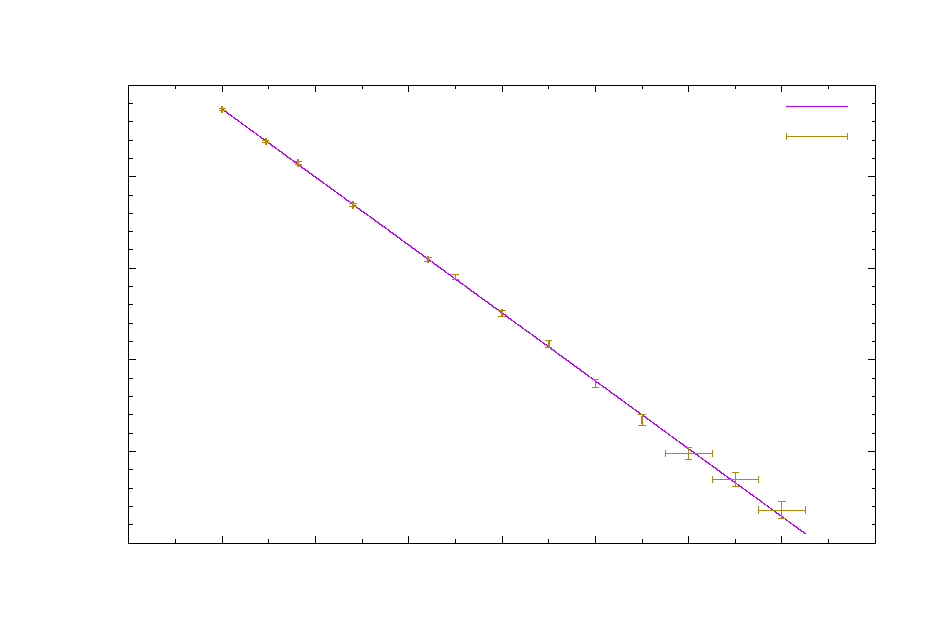
\includegraphics[width={432.00bp},height={288.00bp}]{tv5-plot}}%
    \gplfronttext
  \end{picture}%
\endgroup

		\caption{\centering Entladung einer Kondensators über einen \SI{1}{\mega\ohm} Resistor \captionbr $\chi^2_{\text{red}} = \num{0.476632} \implies$ Gute Anpassung}
		\label{fig:tvfive-plot}
		\vspace{-1em}
	\end{figure}
	Als Endergebnis erhalten wir:
	\begin{equation*}
		\begin{tabu}{lll}
			\toprule
			\text{Variable} & \text{Wert} & \text{Gerundet} \\
			\midrule
			m & \SI{-1.85444(918)}{\per\second} & \SI{-1.854(10)}{\per\second}\\
			c & \SI{1.36878(274)}{} & \SI{1.3688(28)}{} \\
			\bottomrule
		\end{tabu}
	\end{equation*}
	Aus \eqref{fig:tvfive-plot} gilt somit, dass die Relaxationszeit $t_e$ durch:
	\begin{align}
		t_e &= RC = -\frac{1}{m} = -\frac{1}{\SI{-1.854}{\per\second}} = \SI{0.539374}{\second} \sigfig{6} \\
		\Delta t_e &= \abs{\pdv{t_e}{m}\Delta m} = \frac{\Delta m}{m^2} = \frac{\SI{0.010}{\per\second}}{(\SI{-1.854}{\per\second})^2}= 
		\SI{2.90925e-3}{\second}\sigfig{6}
	\end{align}
	gegeben ist. Wir erhalten dann als Relaxationszeit $t_e = \SI{0.539(3)}{\second}$.

	Im Experiment waren einen Widerstand von $\SI{1}{\mega\ohm}$ und einen Kondensator von $\SI{1}{\micro\farad}$ benutzt. Wir erwarten folglich eine Relaxationszeit von $t_e = (\SI{1e6}{\ohm})(\SI{1e-6}{\farad}) = \SI{1}{\second}$.

	Der entsprechende Fehler ist gegeben durch:
	\begin{align}
		\Delta t_e &= t_e \relquad{R, C} = \sqrt{\left(1\%\right)^2+\left(\frac{\SI{e-8}{\farad}}{\SI{1e-6}{\farad}}\right)^2} \notag\\
		&=\SI{0.015}{\farad}
	\end{align}
	Also erhalten wir eine theoretische Relaxationszeit von $t_e = \SI{1.000(15)}{\second}$.
	\begin{center}
		\begin{tabular}{ll}
			\toprule
			Theoretische Wert & \SI{1.000(15)}{\second}\\
			Experimentelle Wert & \SI{0.539(3)}{\second} \\ 
			\bottomrule
		\end{tabular}
	\end{center}
	Im Vergleich ist die erhaltene Relaxationszeit viel kleiner als die erwartete Relaxationszeit, also unterscheiden sich die Werten signifikant voneinander. Das liegt vermütlich daran, dass der effektive Widerstand des Schaltnetz durch die Verwendung vom Tastkopf und Oszilloscope im parallel zum $\SI{1}{\mega\ohm}$ Widerstand verringelt hat. Das wird dann zu einer geringen Relaxationszeit führen, was wir hier tatsächlich beobachtet haben. 

	Wenn man noch Zusatzexperimente machen kann, kann man den Widerstand von Tastkopf charakterisieren, um zu wissen, ob die gemessene Daten mit der Theorie übereinstimmt. 